


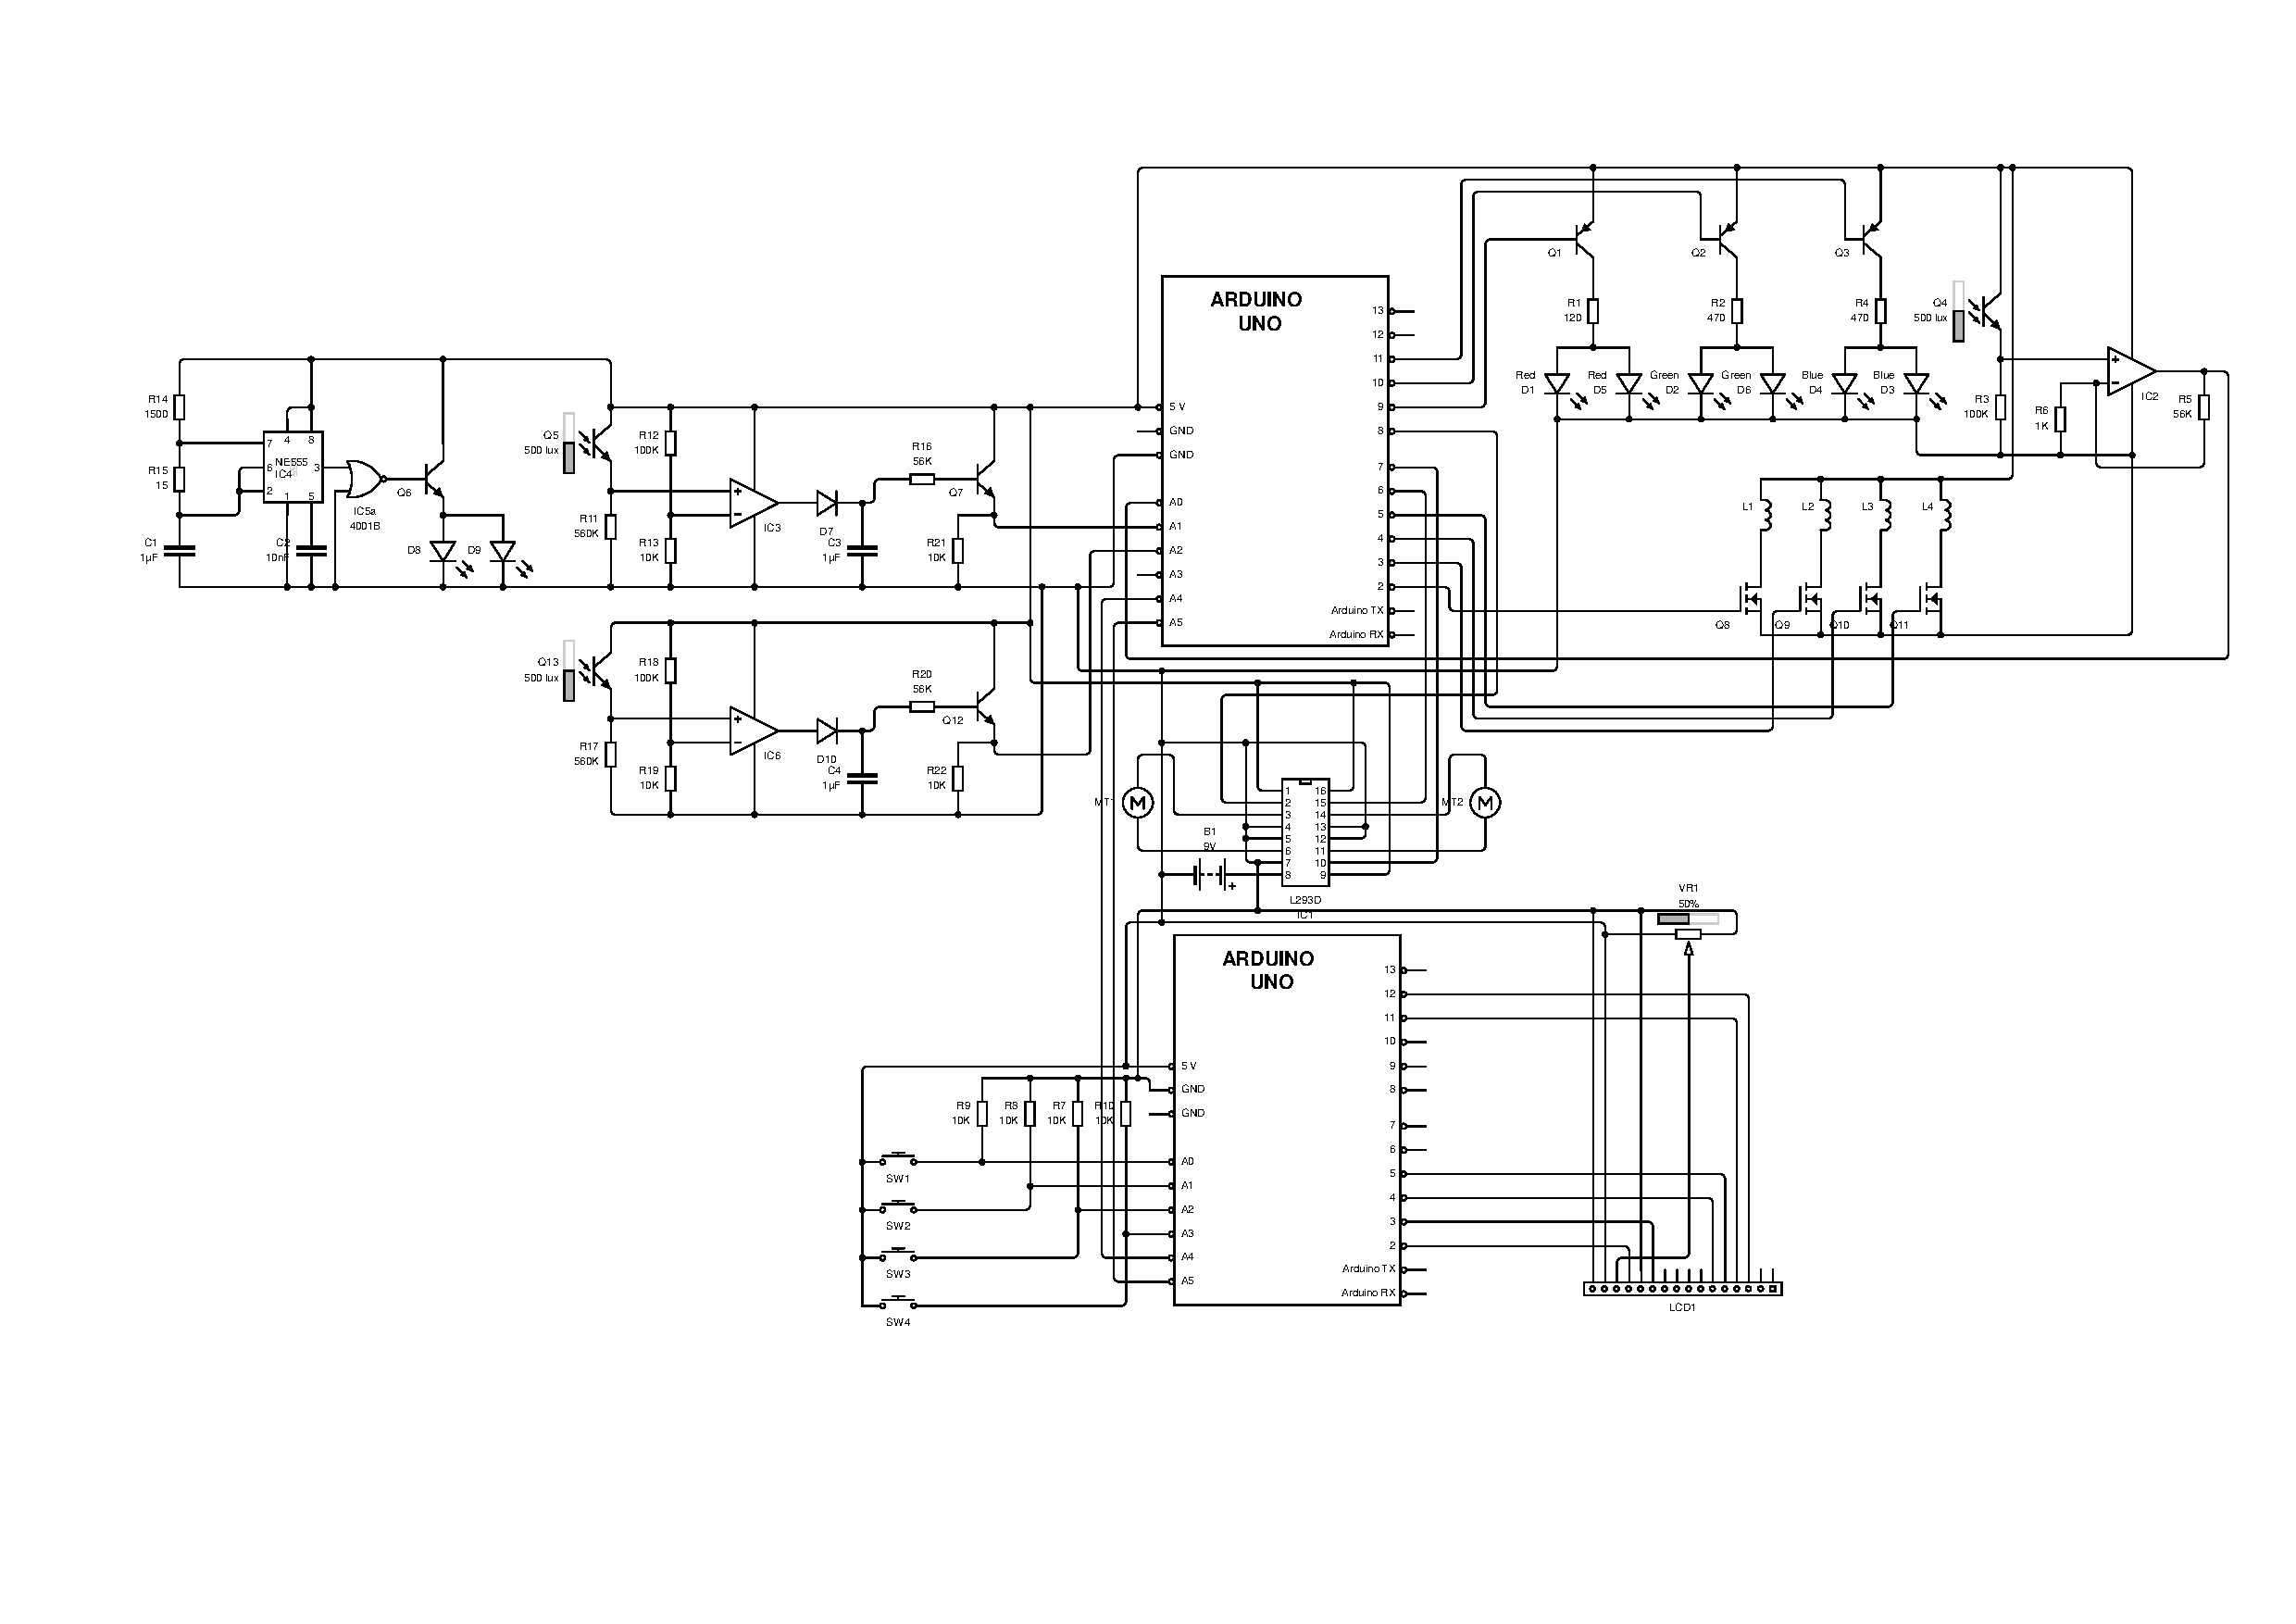
\includepdf[pages=1,fitpaper,pagecommand={\section{Samlet kredsløb} \label{bilag:samletkreds}}]{figures/CIRCUITS/samletFINAL}

% pagecommand={\section{Samlet kredsløb} \label{bilag:samletkreds}}


\section{Endelig prototype - kredsløb} \label{bilag:endeligprotokreds}
\begin{center}
	\includegraphics[width=15cm]{figures/2_5fremstilling/prototyper/Endeligproto.png}
\end{center}

\section{Endelig prototype - kanonkonstruktion} \label{bilag:endeligprotokanon}
\begin{center}
	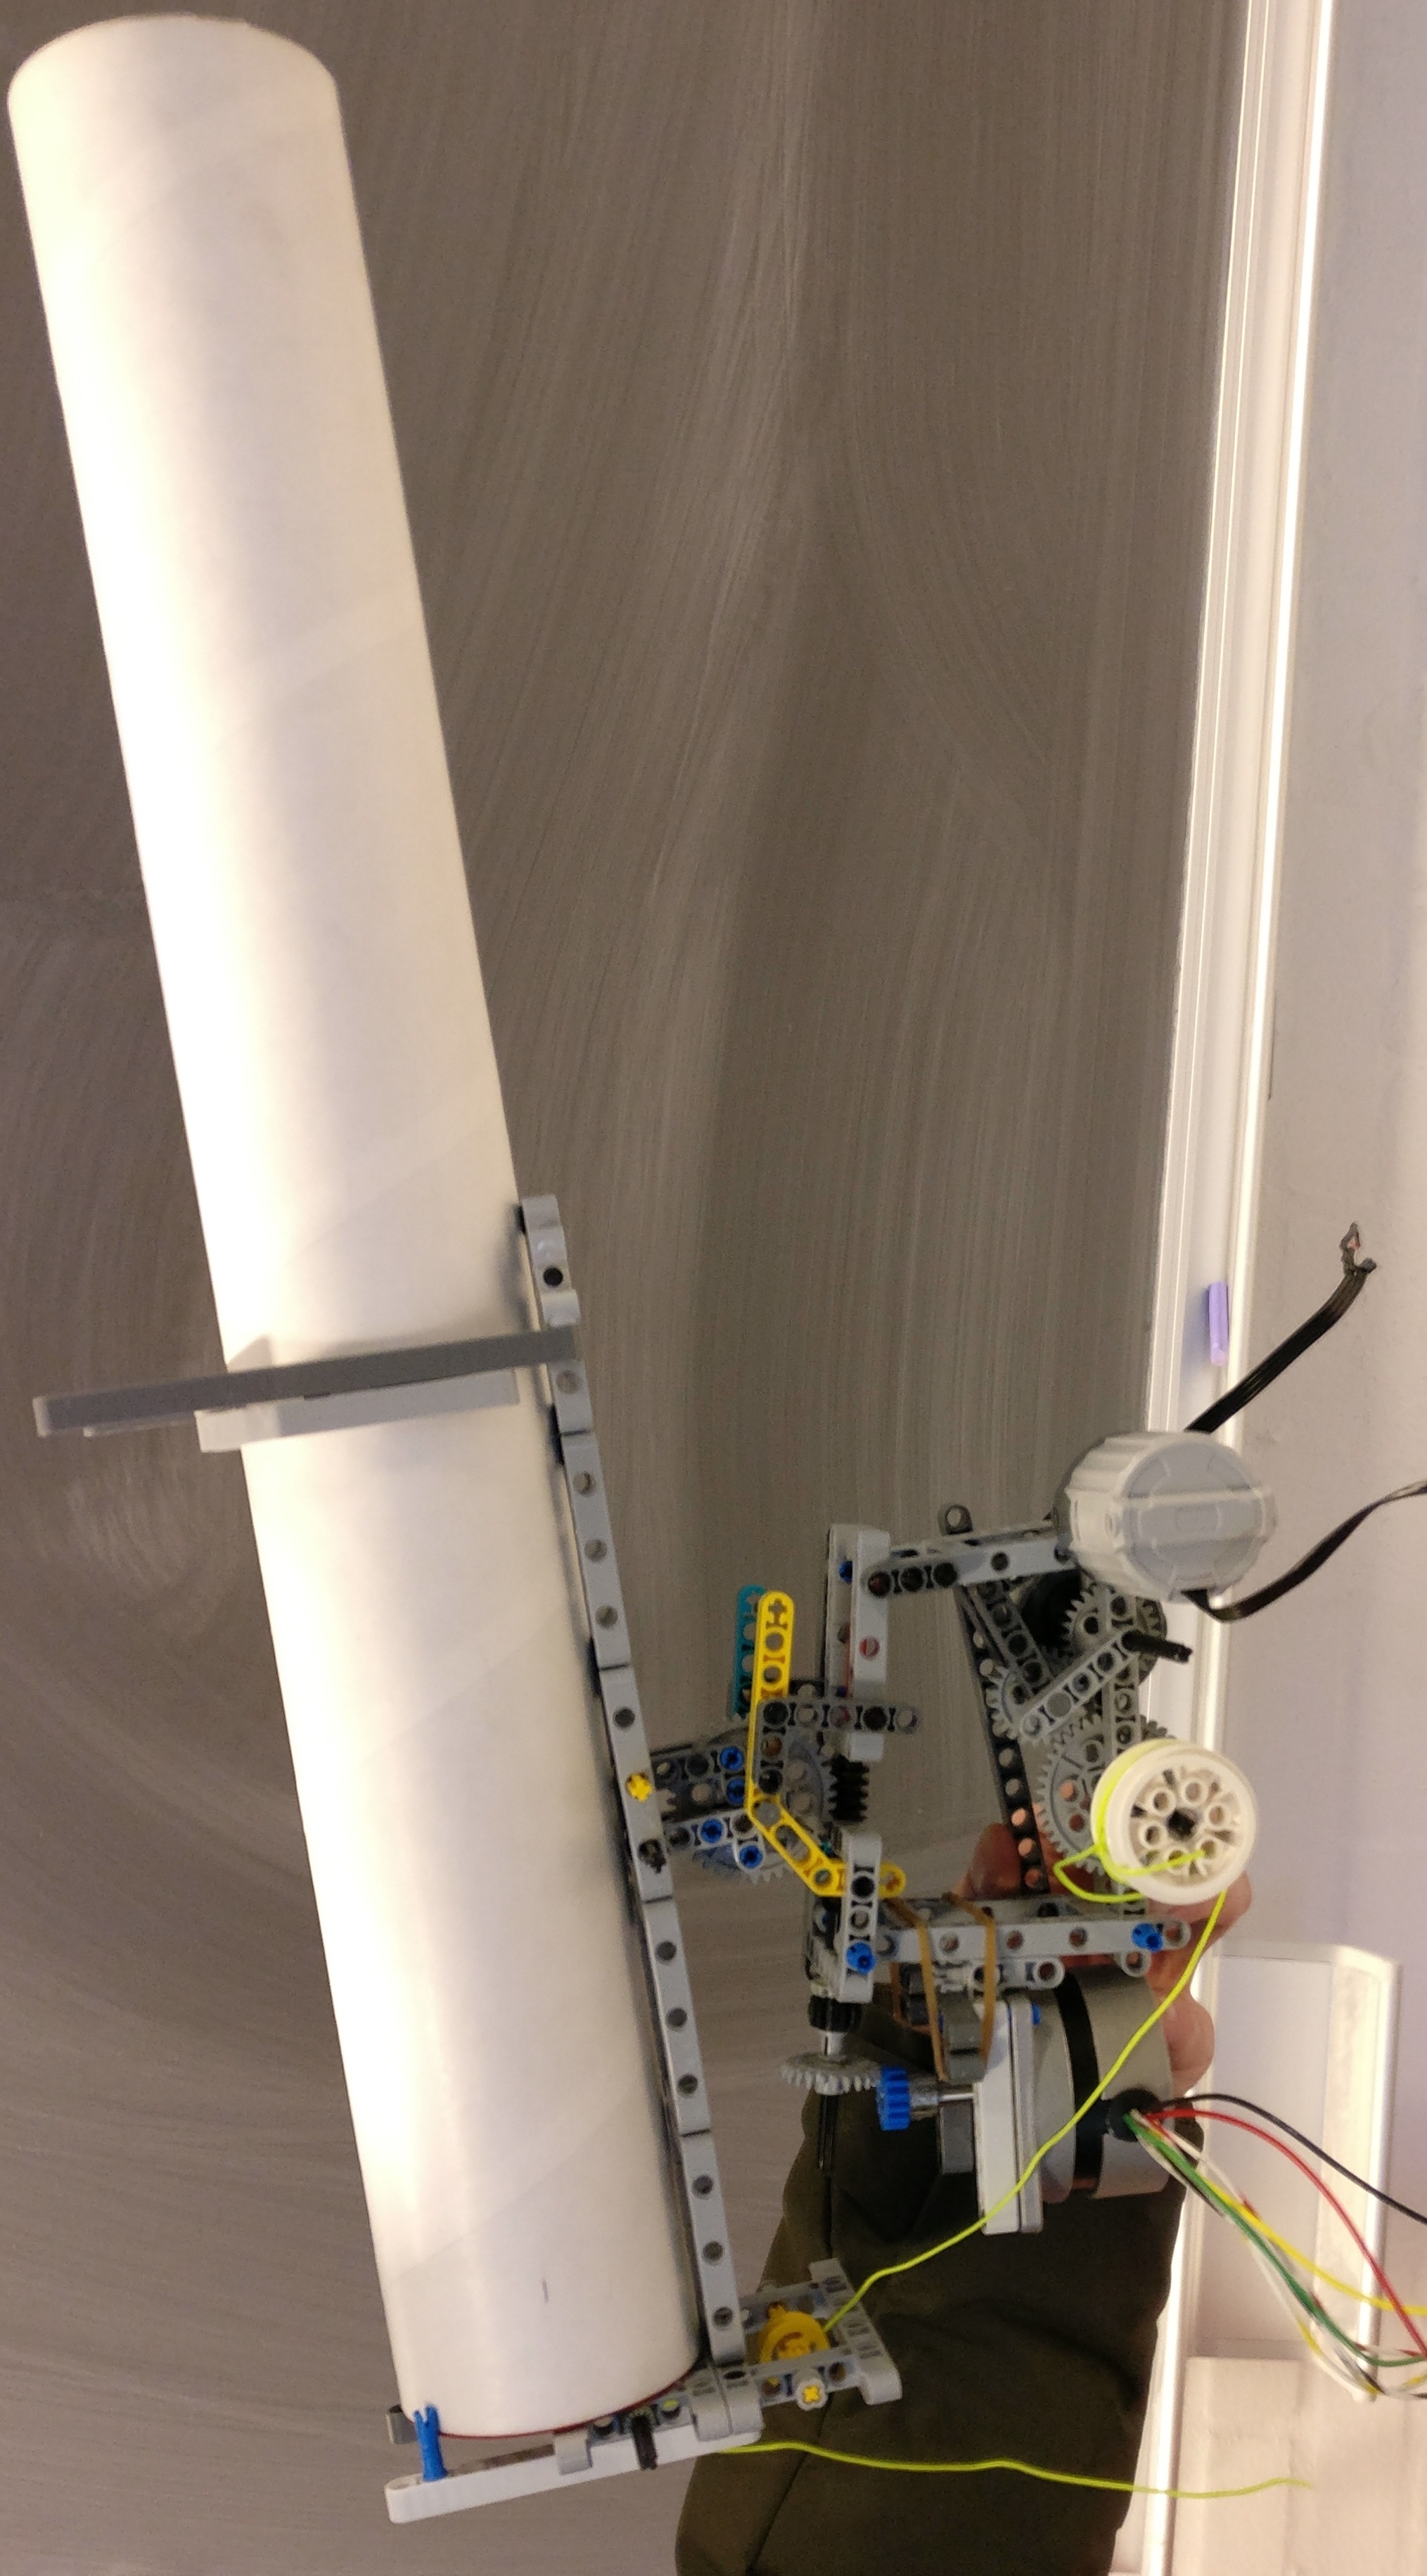
\includegraphics[height=20cm]{figures/2_5fremstilling/prototyper/paenkanon.jpg}
\end{center}
\section{PCB artwork til hastighedssensor}\label{bilag:afsenderModtagerArtwork}
\begin{figure}[H]
	\centering
    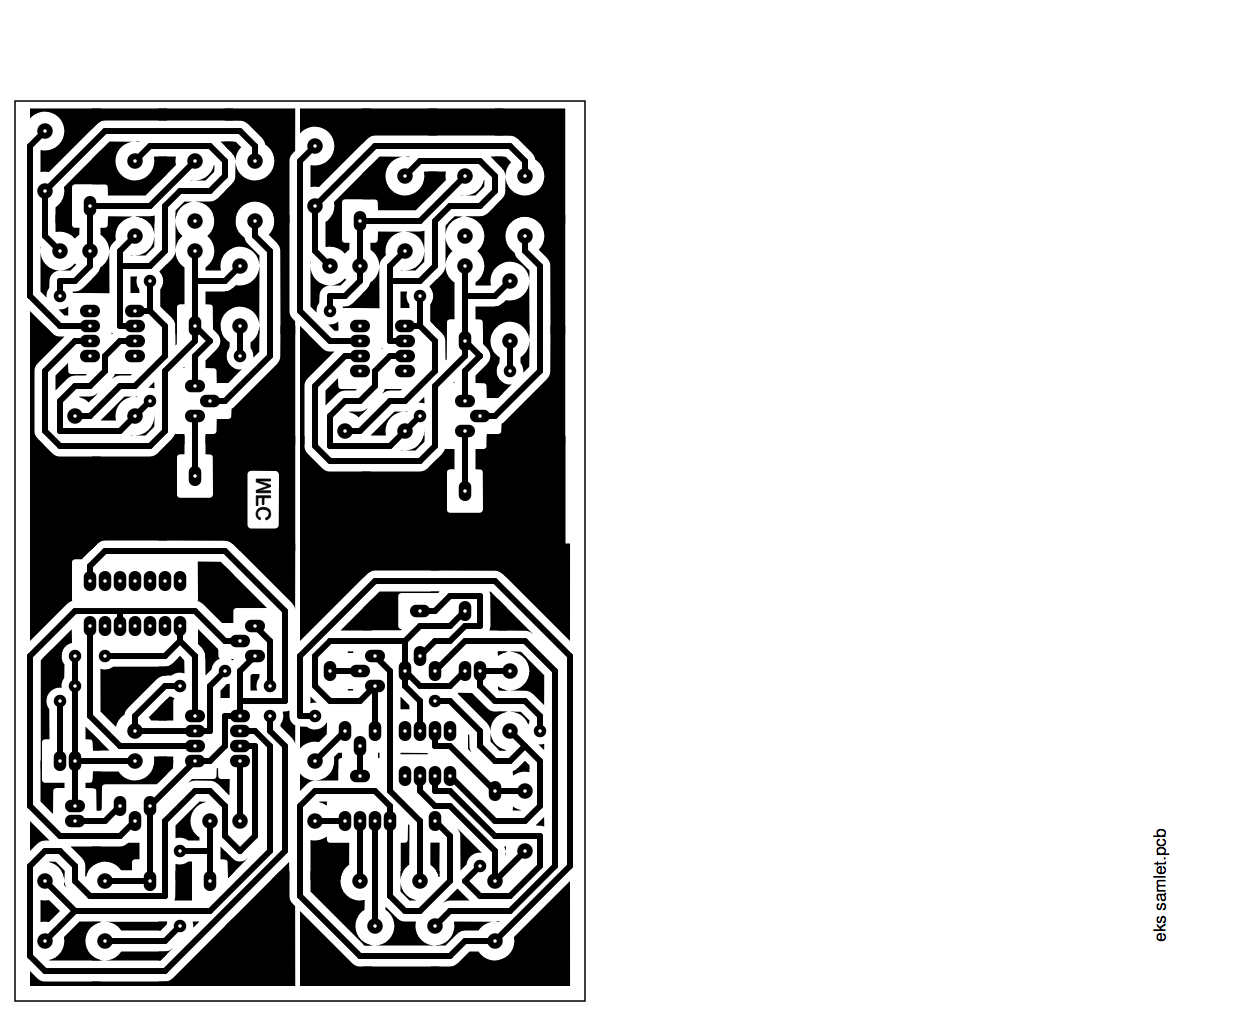
\includegraphics[width=210mm]{figures/2_5fremstilling/afsenderModtagerArtwork.png}
\end{figure}


\section{PCB artwork til arduino shield} \label{bilag:shieldArtwork}
\begin{figure}[H]
	\centering
    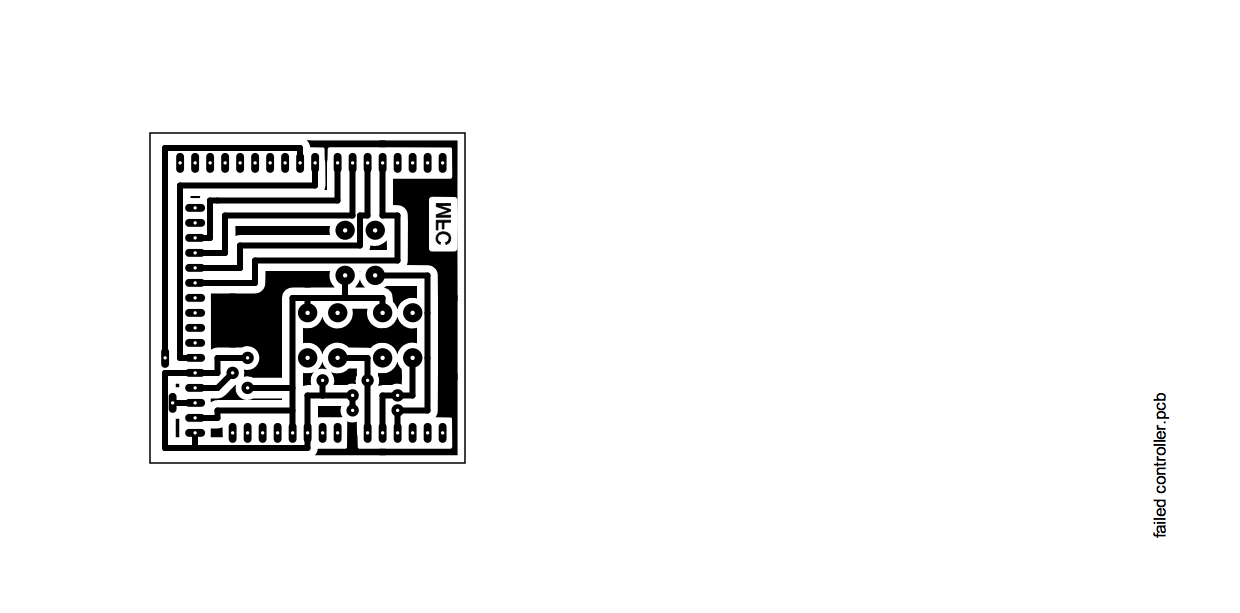
\includegraphics[width=210mm]{figures/2_5fremstilling/shieldArtwork.png}
\end{figure}

\todo{Måske skulle vi overveje at lave et nyt billede med samlede kabler}
\begin{figure}[H]
\section{Fumlebrætmodel anden del}
	\centering
    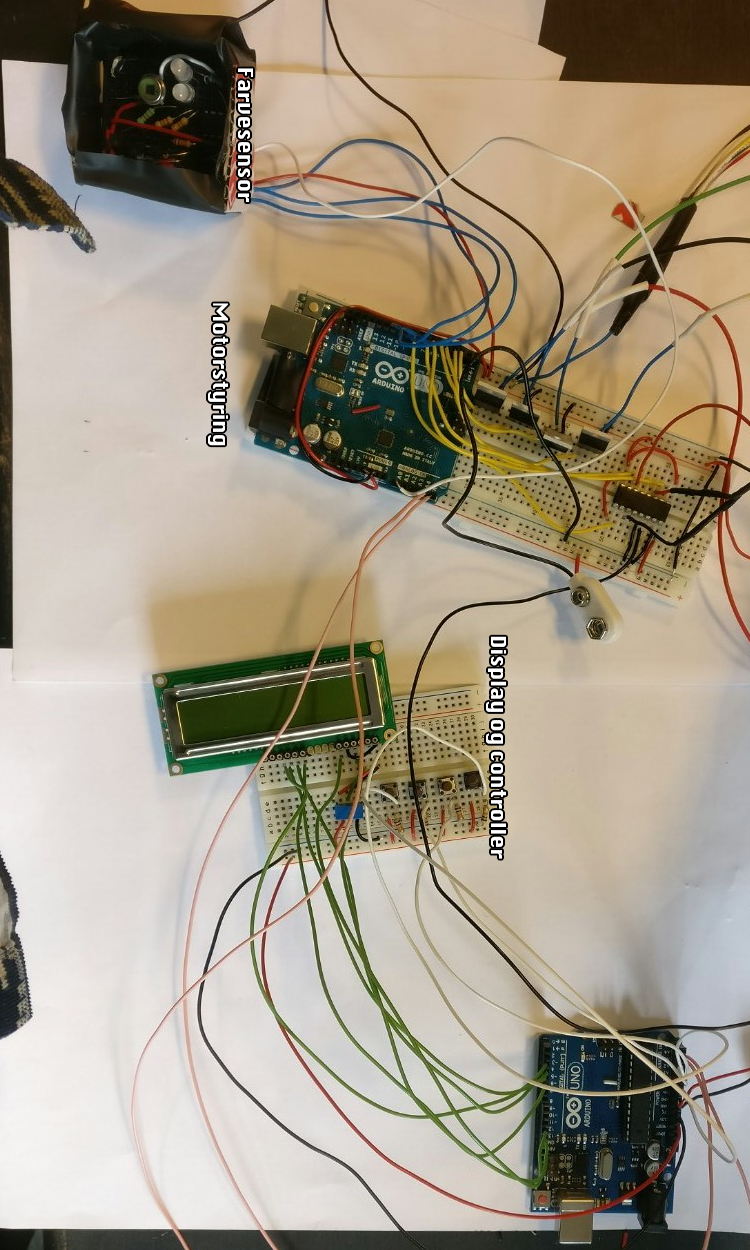
\includegraphics[width=13cm]{figures/2_5fremstilling/prototyper/rumleKreds.png}
\end{figure}

% Must be second last (the longer the later)
\section{Program til Master Arduino}
\label{bilag:programMaster}
\begin{lstlisting}
#include <Wire.h>
#include <Stepper.h>

//Debug funktioner - Hvis debug er defineret vil der komme debug output til serial porten
#define DEBUG //Hvis debug er defineret. Den foerste funktion paa hver linje bliver erstattet med den anden funktion paa linjen, naar programmet bliver kompileret
#ifdef DEBUG
#define DEBUG_PRINTLN(x) Serial.println(x)
#define DEBUG_PRINTLNF(x,y) Serial.println(x,y)
#define DEBUG_PRINT(x) Serial.print(x)
#else //Hvis debug ikke er defineret. Her gaelder det samme, som betyder at funktionerne bliver fjernet
#define DEBUG_PRINTLN(x)
#define DEBUG_PRINTLNF(x,y)
#define DEBUG_PRINT(x)
#endif

//Wire - I2C protokol
int ADDRESS = 9; // Dens egen addresse. Ikke noedvendig, da dette er masteren af netvaerket, men blev sat alligevel
int SLAVEADD = 8; //Addressen til controlleren
char seperatorChar = 254; //ASCII tegnet som bruges til at adskille linjerne i dataen
char modeChar = 50; //ASCII tegnet som indikere at det en farve der skal paa displayet

//LCD variabler
char mode = 0; // Den sidste mode
String colorBuffer; //Den sidste sendte farve
String speedBuffer = "-1m/s"; //Den sidste sendte hastighed
String angleBuffer; //Den sidste sendte vinkel

//Retningsregulerende kreds
int stepperrev = 400; // Antal skridt per omgang
Stepper retning(stepperrev, 2, 3, 4, 5); //vores stepper motor objekt, med de tilsluttede ben og
int gearing = 40; //forholdet mellem hvor meget kannonen rygger sig og stepper motoren drejer
int stepsize = stepperrev * gearing / 180; // Skridtstoerrelsen for naar jystere, er lavet til at dreje 2 grad for hvert tryk
int currangle = 0; //Den nuvaerende vinkel i grader

//Controller
byte states; // det modtaget Port C input registre fra controlleren. Viser state af de forskellige ben
int upbit = 0; //Angiver hvilket bit i byten der tilhoere op knappen. analog A0
int downbit = 1; //Angiver hvilket bit i byten der tilhoere ned knappen. analog A1
int firebit = 2; //Angiver hvilket bit i byten der tilhoere skyd knappen. analog A2

//Hastighed
String Speed = "-1m/s"; //Den beregnede fart som string
int hastpin1 = A1; // Den ene hastighedsensor input ben
int hastpin2 = A2; // Den anden hastighedssensor input ben
float lengthtube = 1; //Laengden imellem de to hastighedssensor i meter

//Farver
boolean newball = true; //Angiver om der er kommet en ny bold i roeret, som betyder at farven skal tjekkes
int confirm; // Antallet af gange som sensoren har bestemt den samme farve
//Dette bliver brugt saa farven bliver bestemt flere gange i traek, og hvis det samme resultat kommer nok gange, antager vi at det den rigtige farve
int confirmAmount = 5; // Antallet af gange den skal faa den samme farve
int pinRGB[] = {12, 11, 13}; //benene til de forskellige LED'er
int pinColorSensor = A0; //Benet hvor farvesensoren er tilsluttet
int lightval[4]; //Et array til at gemme vaerdierne af farvesensoren naar den bliver belyst med forskellig farve. 0 er Roed, 1 er groen, 2 er blaa og 3 er hvid
int fireval = 0; //Angiver hvor haardt bolden skal skydes
String light[] = {"RED", "GREEN", "BLUE", "WHITE"}; //Angiver de forskellige farvers navne
String color; // Den sidste besluttede farve

//Affyringsmekanisme
int gearpinlock = 10; //Benet som vores gear laases paa
int gearpinunlock = 9; //Benet som vores gear laases op paa
int trekpin = 6; //Benet hvor vores traekke motor er paa. Skal kun kunne koere en vej

void setup() {
  //ben tilstanden saettes for vores input og output
  pinMode(gearpinlock, OUTPUT);
  pinMode(gearpinunlock, OUTPUT);
  pinMode(trekpin, OUTPUT);
  pinMode(pinRGB[0], OUTPUT);
  pinMode(pinRGB[1], OUTPUT);
  pinMode(pinRGB[2], OUTPUT);
  pinMode(pinColorSensor, INPUT);
  pinMode(hastpin1, INPUT);
  pinMode(hastpin2, INPUT);

  //Da vi benytter NPN transistor, skal benene saettes hoej for at slukke LED'erne
  digitalWrite(pinRGB[0], HIGH);
  digitalWrite(pinRGB[1], HIGH);
  digitalWrite(pinRGB[2], HIGH);

  //Kommunikationen med I2C starter, med angivet addresse
  Wire.begin(ADDRESS);

  //Serial kommunikation med computeren hvis DEBUG
#ifdef DEBUG
  Serial.begin(9600);
#endif

  //Hastigheden af vores retningsregulerende motor saettes (stepper motoren)
  retning.setSpeed(25);
}

void loop() {
  //Ser om den foerste hastighedssensor er blokeret, hvilket betyder at der er en bold i roeret.
  //Hvis der er det, saa bestem dens farve
  if ((analogRead(hastpin1)) <= 250)determinecolor();
  else {
    //Ellers nulstil vaerdier til naeste bold
    DEBUG_PRINTLN("WAITING FOR BALL");
    newball = true;
    confirm = 0;
  }
  getinput(); //Faa input fra controlleren
  lcddisplay(); //Hvis der er noget nyt der skal paa displayet, saa skriv det til controlleren
}


//Denne funktion modtager en byte fra controlleren, hvori at tilstanden af op, ned og skyd benet er i. Denne funktion finder ud af hvad der skal ske naar de forskellige er trykket
void getinput() {
  Wire.requestFrom(SLAVEADD, 1); //Anmoder om 1 byte data fra controlleren

  //Hvis noget data bliver sendt, saa set det i states
  if (Wire.available()) states = Wire.read();
  else return;

  //Udskriver hvad vi har modtaget binaert
  DEBUG_PRINT("Recieved: ");
  DEBUG_PRINTLNF(states, BIN);

  //Ser om op knappen er trykket, og ned knappen ikke er trykket
  if (bitRead(states, upbit) && !bitRead(states, downbit)) {
    //Hvis den er det, saa skal retningsmotoren koere 1 grad op
    DEBUG_PRINT("Updated angle from ");
    DEBUG_PRINT(angle()); //Funktion til at udskrive vinklen som en string
    DEBUG_PRINT(" to ");
    currangle += 2; //Aendre den nuvaerende vinkel med 2 grad
    DEBUG_PRINT(angle()); //Udskriver den nye vinkel
    DEBUG_PRINTLN();
    retning.step(stepsize); //Saetter retningsmotoren til at koere 2 grad op
  }
  //Ser om op knappen er trykket, og ned knappen ikke er trykket
  if (bitRead(states, downbit) && !bitRead(states, upbit)) {
    //Hvis den er det, saa skal retningsmotoren koere 1 grad ned
    DEBUG_PRINT("Updated angle from ");
    DEBUG_PRINT(angle());
    DEBUG_PRINT(" to ");
    currangle -= 2; //Aendre den nuvaerende vinkel med -2 grad
    DEBUG_PRINT(angle());
    DEBUG_PRINTLN();
    retning.step(-stepsize);//Saetter retningsmotoren til at koere 2 grad ned
  }
  if (bitRead(states, firebit))fire(); //Kalder affyringsfunktionen hvis skyd knappen er trykket
}

// Funktionen som skyder bolden afsted
void fire() {
  DEBUG_PRINTLN("Firing");
  if (!(analogRead(hastpin1) <= 250)) { //Hvis den ene hastighedssensor er hoej, saa er der ikke en bold i roeret, som betyder at affyringen skal stoppes
    DEBUG_PRINTLN("NOT LOADED");
    return;
  }
  if (newball) { //Hvis boldens farve stadig ikke er bekraeftet, saa stop affyringen
    DEBUG_PRINTLN("COLOR NOT VERIFIED");
    return;
  }
  //Skriver indstillingen (farven) til Serialporten
  DEBUG_PRINT("Setting: ");
  DEBUG_PRINTLN(color);

  long time = millis(); //den nuvaerende tid i millis
  digitalWrite(trekpin, HIGH); //Saetter traek bennet hoej, saa elastiken bliver strukket ud
  digitalWrite(gearpinlock, 130); //Saetter den i gear
  while (millis() - time <= fireval * 1000); // Treaker i det stykke tid der svare til indstillingen
  // Der laases nu op, ved at saette den i frigear
  DEBUG_PRINTLN("UNLOCKING");
  digitalWrite(gearpinlock, LOW);
  digitalWrite(gearpinunlock, 130); //traekker gearet ud i frigear
  digitalWrite(trekpin, LOW);

  time = millis(); //Vi opdatere tiden
  determinespeed(); //Funktionen der bestemmer boldens hastighed
  while (millis() - time <= 2000); //Saa laenge der ikke er gaaet 2 sekunder, saa vent, Dette er for at soerge for at gearet bliver holdt i frigear i lang nok tid
  digitalWrite(gearpinunlock, LOW); //Stopper med at holde gearet fast i frigear
}


String angle() { //Returnere vinklen som en string
  return String(currangle);
}

void determinecolor() {// Bestemmer farven af bolden i roeret
  if (!newball) return; // Hvis farven alleree er bestem og bekraeftet, saa lad vaere med at tjekke farven
  DEBUG_PRINTLN("DETERMINE COLOR");
  //Taender for alle farverne
  for (int i = 0; i < 3; i++) {
    digitalWrite(pinRGB[i], LOW);
  }
  delay(10);
  lightval[3] = analogRead(pinColorSensor); //gemmer farvesensorens vaerdi i lightval[3]
  //slukker alle LED'erne igen
  for (int i = 0; i < 3; i++) {
    digitalWrite(pinRGB[i], HIGH);
  }

  if (lightval[3] > 770) { //Hvis spaendingen er hoejere end 3.8 V er bolden hvid
    setColor(light[3], 1); //Saetter farven til hvid
    return;
  }

  for (int i = 0; i < 3; i++) {//Gaar igennem alle LEDerne og taender og slukker dem en efter en, og gemmer farvesensor vaerdien
    digitalWrite(pinRGB[i], LOW); //Taender for LEDen
    delay(10);
    lightval[i] = analogRead(pinColorSensor); //gemmer vaerdien i lightval
    DEBUG_PRINT(light[i]);
    DEBUG_PRINT(" Value: ");
    DEBUG_PRINTLN(lightval[i]);
    digitalWrite(pinRGB[i], HIGH); //slukker LEDen igen
  }

  if (lightval[0] * 1.2 > lightval[1] && lightval[0] * 1.2 > lightval[2]) { //Tjekker om farven er roed
    setColor(light[0], 2); //Saetter farven til roed og skydevardien til 2
    return;
  }
  if (lightval[1] > lightval[2] && lightval[1] > lightval[0]) { //Tjekker om farven er groen
    setColor(light[1], 3); //Saetter farven til roed og skydevardien til 3
    return;
  }
  if (lightval[2] > lightval[0] && lightval[2] > lightval[1]) { //Tjeker om farven er blaa
    setColor(light[2], 4); //Saetter farven til roed og skydevardien til 4
    return;
  }
}

void setColor(String newColor, int newFireval) { // Denne funktion saetter farven, og tjekker bekraeftelse
  if (color == newColor) {  //Hvis den forrige bold var samme farve, saa skal confirm blive 1 hoejere
    confirm += 1;
    if (confirm == confirmAmount)newball = false; //Hvis antallet af gange boldens farve er blevet bekraeftet, saa saet newball falsk
  } else { // Ellers genstart bekraeftelses processen og saet farven til newColor
    confirm = 0;
    color = newColor;
  }
  fireval = newFireval; //Tiden som elastikken skal blive traekket i bliver sat til newFireval
  DEBUG_PRINT("COLOR DETECTED : ");
  DEBUG_PRINTLN(color); //Skriver den fundede farve til Serialporten
}

void determinespeed() { // Bestemmer hastigheden af bolden
  DEBUG_PRINTLN("DETERMING SPEED");
  unsigned long time = millis(); //den nuvaerende tid saettes i time
  long calc; //en vaerdi til at se hvornaar den foerste hastighedssensor kan se bolden
  while (millis() - time <= 3000 && !(analogRead(hastpin1) <= 250)); //Venter til den foerste hastighedssensor bliver blokeret eller der er gaeet 3 sekunder
  calc = millis(); //saetter calc til den nuvaerende tid
  while (millis() - time <= 3000 && !digitalRead(hastpin2)); //Venter til den anden hastighedssensor bliver blokeret eller der er gaet 3 sekunder fra funktionen startede
  if (millis() - time >= 3000) { //tjekker om der er gaaet 3 sekunder, som betyder at der er TIMEOUT
    return;
  }
  Speed = String(lengthtube / (((float)(millis() - calc)) / 1000.0), 1); //Beregner hastigheden og laver det om til en String med 1 decimal precision
  Speed += "m/s";
  DEBUG_PRINTLN("Updated speed: " + Speed);
}

void lcddisplay() {//Opdatere displayet
  String data; //Stringen som skal sendes. Denne bliver bygget paa igennem funktionen
  boolean changed = false; //Angiver om noget har aendret sig paa displayet siden den sidst blev opdateret
  //Ser om farven har aendret sig
  if (colorBuffer != color) {
    mode = modeChar; //tilstanden bliver sat til farv
    data += mode; //saetter moden paa data stringen
    colorBuffer = color; //laver farve bufferen om til den nuvaerende farve
    data += colorBuffer; //saetter farvebufferen paa data stringen
    changed = true; //Angiver at noget har aendret sig
  }
  //Ser om hastigheden har aendret sig
  else if (speedBuffer != Speed) {
    mode = modeChar + 1; //tilstanden bliver sat til hastighed (noget andet end modeChar)
    data += mode; //Saetter moden paa data stringen
    speedBuffer = Speed; //Laver hastighedsbufferen om til den nuvaerende hastighed
    data += speedBuffer; //Saetter hastighedsbufferen paa data stringen
    changed = true; //angiver at noget har aendret sig
  } else { //Ellers fyldes data stringen op med de sidst gemte vaerdier. Detter er vist anden linje skal opdateres
    data += (char)mode;
    if (mode == modeChar)data += colorBuffer;
    else data += speedBuffer;
  }
  data += seperatorChar; //Saetter en seperator paa enden af data stringen
  if (angleBuffer != angle() || changed) {// Hvis vinklen ikke er den samme eller hvis foerste linje har andret sig
    angleBuffer = angle(); //Saetter vinkelbufferen til den nuvaerende vinkel
    data += angleBuffer; //Saetter vinkelbufferen paa data stringen
    changed = true; //Angiver at noget har aendret sig
  }
  data += seperatorChar;//Saetter endnu et seperationstegn
  if (changed) { //Hvis noget har aendret sig
    DEBUG_PRINT("TRANSMITTING: ");
    DEBUG_PRINTLN(data);

    //Laver data stringen om til et array af char
    char dataBuffer[data.length()];
    data.toCharArray(dataBuffer, data.length());

    //Begynder kommunikation til controlleren, og overfoere dataen som et char array
    Wire.beginTransmission(SLAVEADD);
    Wire.write(dataBuffer);
    Wire.endTransmission();
  }
  delay(100); //Venter i 0.1 sekund for at forhindre overbelastning af I2C bufferen
}
\end{lstlisting}

\section{Program til Controller Arduino}
\label{bilag:programController}
\begin{lstlisting}
#include <LiquidCrystal.h>
#include <Wire.h>


//Debug funktioner - Hvis debug er defineret vil der komme debug output til serial porten
#define DEBUG
#ifdef DEBUG //Hvis debug er defineret. Den foerste funktion paa hver linje bliver erstattet med den anden funktion paa linjen, naar programmet bliver kompileret
#define DEBUG_PRINTLN(x) Serial.println(x)
#define DEBUG_PRINTLNF(x,y) Serial.println(x,y)
#define DEBUG_PRINT(x) Serial.print(x)
#else //Hvis debug ikke er defineret. Her gaelder det samme, som betyder at funktionerne bliver fjernet
#define DEBUG_PRINTLN(x)
#define DEBUG_PRINTLNF(x,y)
#define DEBUG_PRINT(x)
#endif

//Wire - I2C protokol
int ADDRESS = 8; // Dens egen addresse. Denne skal bruges naar master vil kontakte controlleren
char seperatorChar = 254; // ASCII tegnet som bruges til at adskille linjerne i dataen
char modeChar = 50; //ASCII tegnet som indikere at det en farve der skal paa displayet

//knapper til controlleren. Benene bliver kun brugt til at angive at det er input, ellers benyttes port manipulation (PINC) til at sende benenes tilstande som en byte.
int uppin = A0;
int downpin = A1;
int skydpin = A2;

//LCD variabler
LiquidCrystal lcd(12, 11, 5, 4, 3, 2); //vores LCD objekt, med benene som den er koblet paa
String line1_const1 = "Farve: "; //Den ene konstant paa linje 1. Skal have et mellemrum efter, da .length bliver brugt
String line1_const2 = "Fart: "; //Den anden konstant paa linje 1. Der skiftes mellem disse med mode i modtager funktionen
String line2_const = "Vinkel: "; //Den ene konstant paa linje 2.


void setup() {
  //ben tilstand for knapperne saettes som input
  pinMode(uppin, INPUT);
  pinMode(downpin, INPUT);
  pinMode(skydpin, INPUT);

  //Starter I2C kommunikation
  Wire.begin(ADDRESS); //Angiver addresse og begynder
  Wire.onRequest(requestEvent); //Angiver funktion der skal kaldes naar controlleren bliver bedt om at sende
  Wire.onReceive(receiveEvent); //Angiver funktion der skal kaldes naar controlleren skal modtage

  //Starter LCD
  lcd.begin(16, 2); //Begynder LCD'en med 2 linjer og 16 tegn per linje
  lcd.print(line1_const1); //Skriver 1. linje konstant paa LCD
  lcd.setCursor(0, 1); //Skifter position til 2. linje
  lcd.print(line2_const); //Skriver 2. linje konstant paa LCD

  //Starter serialkommunikation hvis DEBUG er defineret
#ifdef DEBUG
  Serial.begin(9600);
#endif
}
// Loop funktionen, controlleren skal ikke goere noget hvis den ikke bliver bedt om det
void loop() {
}

//Naar controlleren skal sende data
void requestEvent() {
  byte data = PINC; //Port C input registret
  //Skriver den sendte data binaert i serialkommunikationen hvis DEBUG er defineret
  DEBUG_PRINT("TRANSMITTING DATA: ");
  DEBUG_PRINTLNF(data, BIN);
  DEBUG_PRINTLN();

  Wire.write(data); //Sender dataen over I2C
}

//Naar controlleren modtager data
void receiveEvent(int datalength) {
  DEBUG_PRINTLN("RECIEVING DATA: ");

  boolean mode = (Wire.read() == modeChar ); //Den foerste byte indikere tilstand, hvor at den enden kan vaere 0 eller hoejere end 0

  //Stringene for den 1. og 2. linje
  String firstLineBuffer = getLine(); //Faar den 1. linje fra I2C bufferen
  String secondLineBuffer = getLine(); //Faar den 2. linje fra I2C bufferen

  setDisplay(mode, firstLineBuffer, secondLineBuffer); // Det modtaget data bliver sendt til funktionen setDisplay, som skriver dataen til displayet
}

//Denne funktion laeser fra I2C bufferen indtil at den er tom eller at ny linje tegnet dukker op. Dette bliver sat i en String som bliver returneret
String getLine() {
  String output;
  while (Wire.available()) {//Saa laenge der er noget i I2C bufferen
    char c = Wire.read(); //laes det naeste tegn
    if (c == seperatorChar) break; //Hvis tegnet er seperationstegnet, stop med at laese fra bufferen
    DEBUG_PRINT(c); //Skriv til Serial hvis DEBUG
    output += c; //Ellers skal tegnet tilfoejes til output
  }
  DEBUG_PRINTLN();
  return output; //returner outputtet
}

//opdatere displayet
void setDisplay(boolean mode, String line1, String line2) {

  //Debug udskrivning. Skriver hvad displayet bliver opdateret til
  DEBUG_PRINT("Updating display:  ");
  DEBUG_PRINT("Line 1: ");
  DEBUG_PRINT(line1);
  DEBUG_PRINT("    ");
  DEBUG_PRINT("Line 2: ");
  DEBUG_PRINTLN(line2);
  lcd.clear(); //Fjerner alt fra displayet
  lcd.setCursor(0, 0); //Saetter position til starten af displayet paa 1. linje
  int leng; //laengde paa 1. linje. Dette bruges til at goere resten af felterne tomme paa linjen tomme

  // Skriver konstanten paa 1. linje, alt efter hvilken mode det er (hastighed/farve)
  if (mode) {
    lcd.print(line1_const1);
    leng += line1_const1.length();
  }
  else {
    lcd.print(line1_const2);
    leng += line1_const2.length();
  }

  lcd.print(line1); // Skriver dataen til linje 1 paa linje 1.
  lcd.setCursor(0, 1); // Saetter positionen til 2. linje efter konstanten
  lcd.print(line2_const);
  lcd.print(line2); //Skriver dataen til linje 2 paa linje 2.
}
\end{lstlisting}



% MUST BE LAST
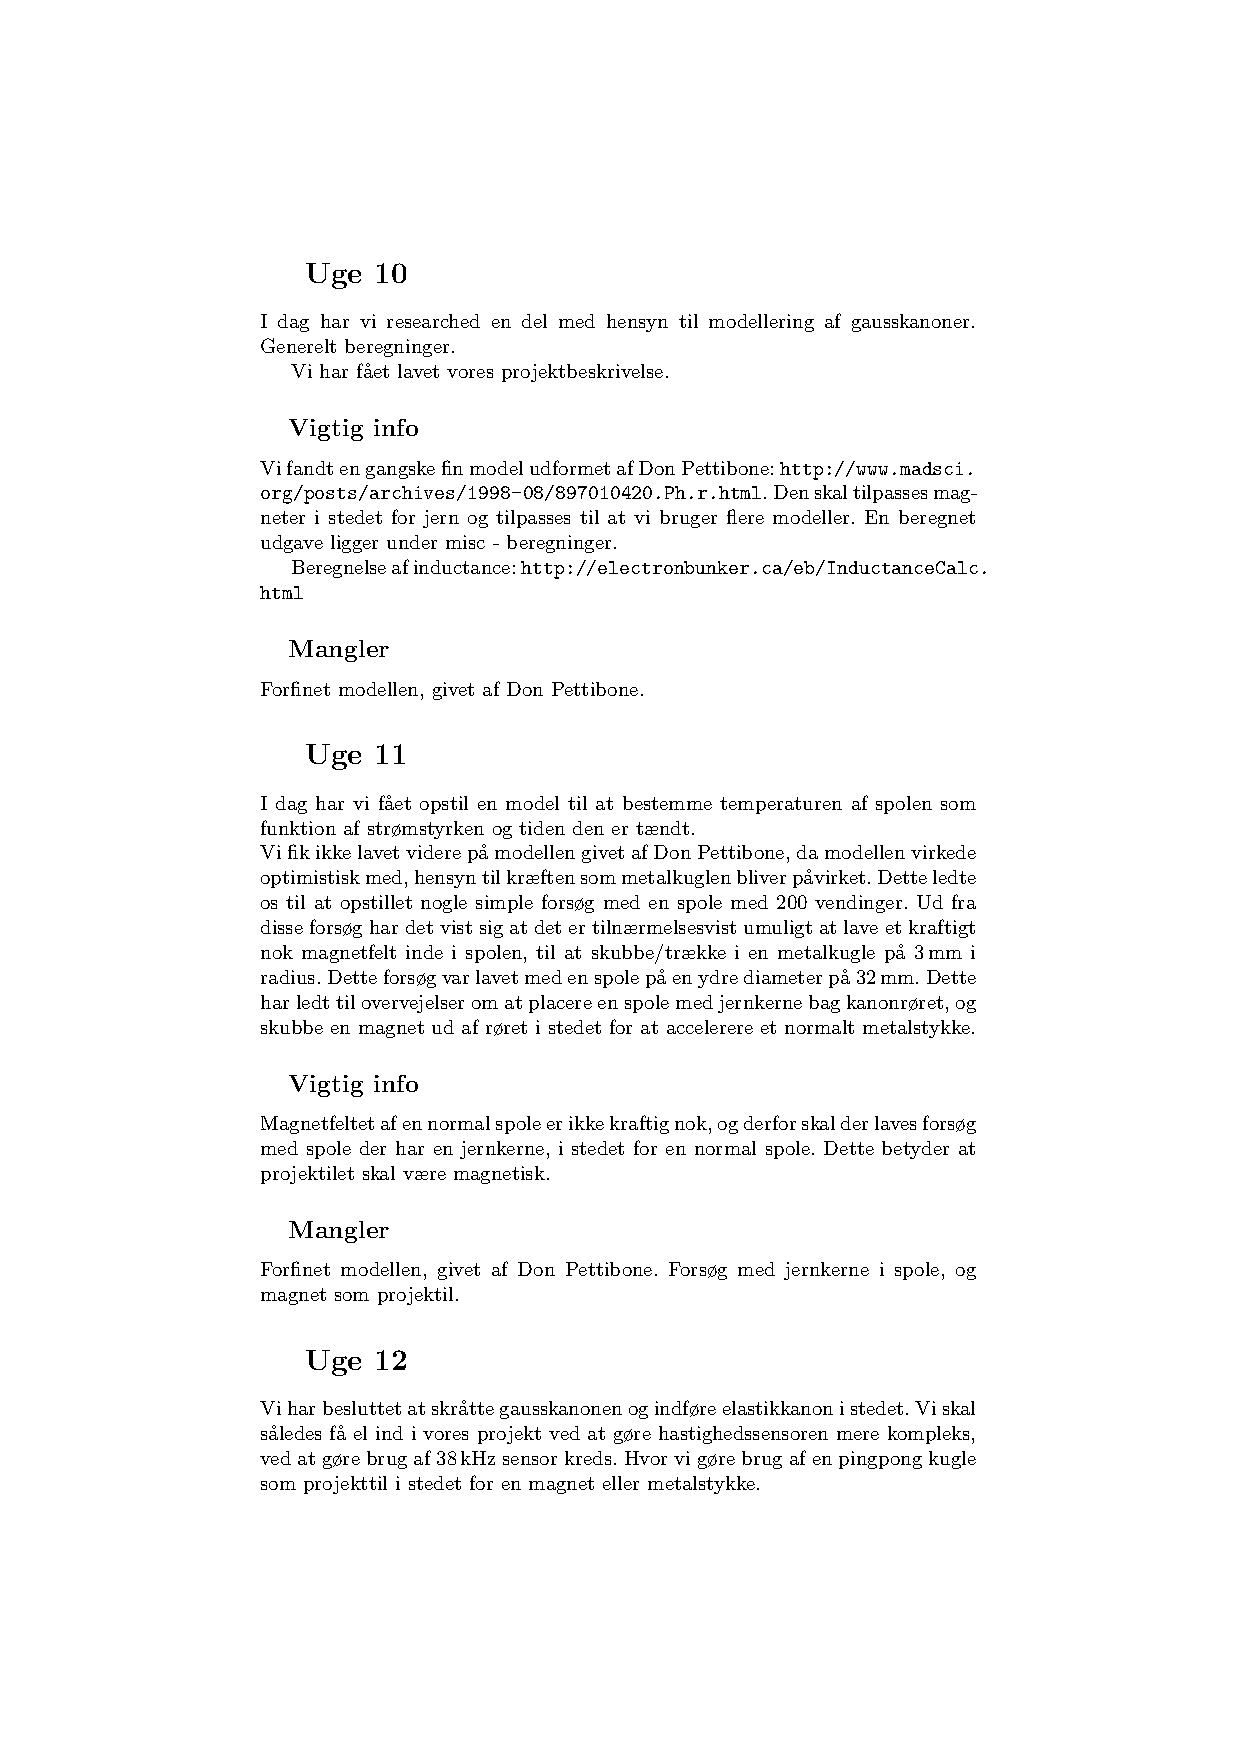
\includepdf[pages = 1, pagecommand = \section{Logbog} \label{bilag:logbog}]{figures/logbog.pdf} 
\includepdf[pages = 2-, pagecommand={}]{figures/logbog.pdf} 

